\chapter{Real-Valued Neural Networks (RVNN)}

While deep learning approaches have successfully demonstrated the profound capability to jointly optimize PAPR reduction and signal recovery, many existing neural network architectures rely on tens of millions of trainable parameters to map signals in the frequency domain. This massive computational footprint presents a severe bottleneck for real-time inference and practical hardware deployment in time-sensitive communication systems.

To address this critical barrier, this chapter explores the low-complexity framework proposed by Liu et al.~\cite{liu2020low}. Rather than learning a high-dimensional mapping across all subcarriers, this framework shifts the neural network processing directly into the \emph{time domain}. By operating strictly on the real and imaginary components of the post-IFFT OFDM waveform using lightweight Real-Valued Neural Networks (RVNN), this approach drastically reduces the required network size.

The proposed architecture consists of two cooperative, highly compact modules:
\begin{itemize}
    \item \textbf{PAPR Reduction Module} operating on the time-domain signal at the transmitter side.
    \item \textbf{PAPR Decompression Module} operating at the receiver side to reconstruct the original waveform.
\end{itemize}

By jointly training these two modules, this time-domain approach aims to achieve highly competitive PAPR reduction and Bit Error Rate (BER) performance while maintaining a minimal computational footprint.

\section{Proposed Neural Network Based PAPR Reduction Method}

The proposed method introduces a collaborative neural-network-based framework consisting of two modules:

\begin{figure}[H]
    \centering
    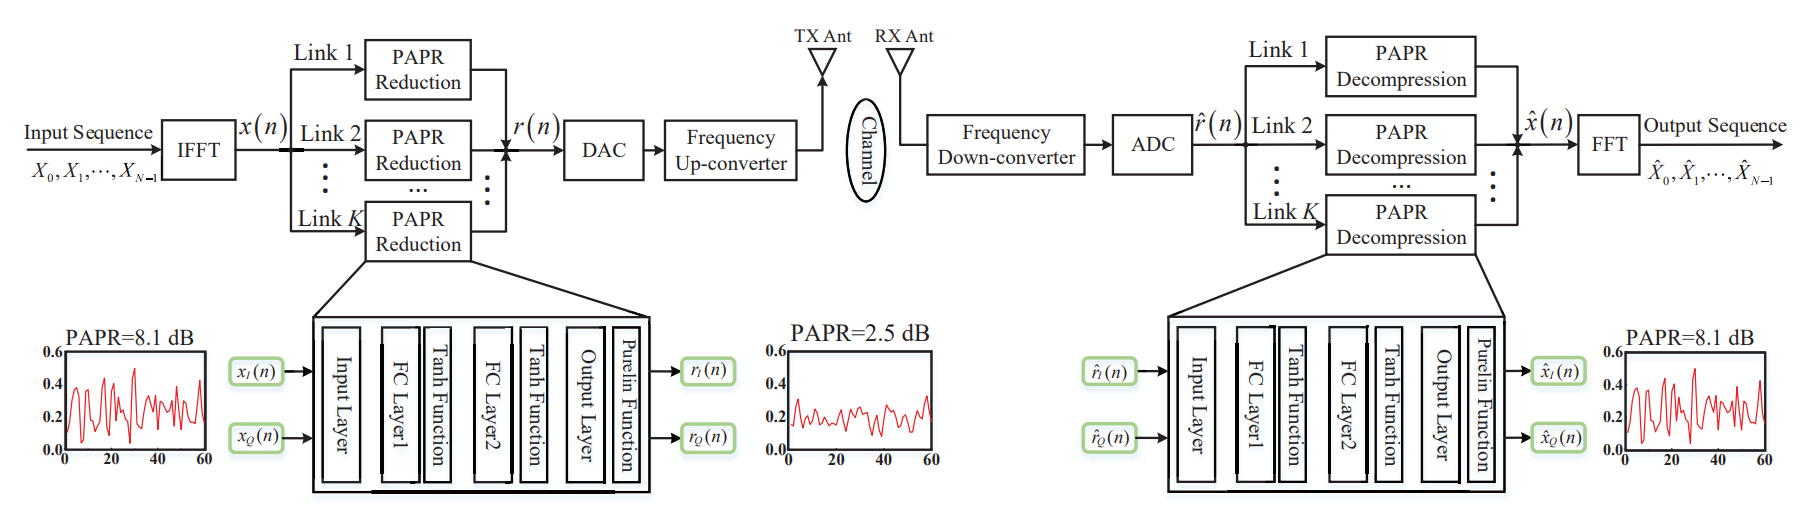
\includegraphics[width=0.95\linewidth]{Figures/RVNN/rvnn_system_model.png}
    \caption{The structure of the proposed model based on real-valued NN}
    \label{fig:system_model}
\end{figure}

\subsection{PAPR Reduction Module}

The reduction module is implemented using a real-valued neural network operating in the time domain. Unlike conventional clipping-based approaches, the proposed neural network learns the nonlinear relationship between the original OFDM signal and its low-PAPR representation through a training process. The objective of the reduction module is to suppress large signal peaks while preserving the information carried by the OFDM symbols.

After the Inverse Fast Fourier Transform (IFFT) operation, the OFDM signal becomes a complex-valued time-domain signal represented as

\begin{equation*}
    x(n)=x_I(n)+j x_Q(n)
\end{equation*}

where $x_I(n)$ and $x_Q(n)$ denote the in-phase (I) and quadrature (Q) components of the OFDM signal, respectively. Since the proposed neural network is real-valued, the complex OFDM signal cannot be directly processed. Therefore, the signal is separated into its real and imaginary components and represented as

\begin{equation*}
    x_n=[x_I(n),x_Q(n)]^T
\end{equation*}

The vector $x_n$ is then used as the input to the neural network.

The proposed neural network architecture consists of four layers:

\begin{itemize}
    \item Input Layer
    \item Fully Connected Layer 1
    \item Fully Connected Layer 2
    \item Output Layer
\end{itemize}

The input layer receives the I/Q components of the OFDM signal and forwards them to the hidden layers without performing any computations. The main feature extraction and nonlinear transformation operations are performed in the fully connected (FC) layers.

In a fully connected layer, each neuron is connected to all neurons in the previous layer. The output of each FC layer is calculated using a weighted summation followed by a nonlinear activation function. Mathematically, the operation of the FC layer can be expressed as

\begin{equation*}
    y_{FC}=f_{FC}(Wx+b)
\end{equation*}

where $W$ denotes the weight matrix, $b$ represents the bias vector, and $f_{FC}(\cdot)$ is the activation function.

The first fully connected layer learns low-level signal characteristics such as amplitude distribution and peak locations in the OFDM waveform. The second fully connected layer performs deeper feature extraction and learns how to suppress high peaks while maintaining signal recoverability.

To improve the nonlinear modeling capability of the network, the hyperbolic tangent activation function (\texttt{tanh}) is employed in the hidden layers. The tanh function maps the input values into the range $[-1,1]$ and can be expressed as

\begin{equation*}
    \tanh(x)=\frac{e^x-e^{-x}}{e^x+e^{-x}}
\end{equation*}

The tanh activation function is selected because OFDM signals contain both positive and negative values, making zero-centered activation more suitable for stable training and faster convergence compared to non-symmetric activations like ReLU.

After passing through the hidden layers, the extracted features are combined in the output layer to generate the low-PAPR OFDM signal. The output of the reduction module is expressed as

\begin{equation*}
    [r_I(n),r_Q(n)]^T=f(x_n,\theta_f)
\end{equation*}

where $f(\cdot)$ represents the nonlinear mapping learned by the neural network and $\theta_f$ denotes the trainable parameters of the reduction network, including weights and biases.

Finally, the real and imaginary outputs are recombined to form the complex-valued low-PAPR OFDM signal

\begin{equation*}
    r(n)=r_I(n)+j r_Q(n)
\end{equation*}

The generated signal $r(n)$ is then transmitted through the wireless communication channel. By learning the optimal nonlinear transformation, the proposed reduction module effectively decreases the Peak-to-Average Power Ratio while minimizing signal distortion and preserving communication reliability.

\subsection{PAPR Decompression Module}

At the receiver side, a PAPR decompression module is employed to reconstruct the original OFDM signal from the received low-PAPR signal. Since the PAPR reduction process modifies the transmitted signal to suppress large peaks, some distortion may be introduced during transmission. Therefore, the decompression module is designed to recover the original OFDM signal and minimize the Bit Error Rate (BER) degradation.

After transmission through the wireless channel, the received signal passes through the down-conversion and Analog-to-Digital Converter (ADC) stages. The received signal can be represented as

\begin{equation*}
    \hat{r}(n)=\hat{r}_I(n)+j\hat{r}_Q(n)
\end{equation*}

where $\hat{r}_I(n)$ and $\hat{r}_Q(n)$ denote the in-phase and quadrature components of the received signal, respectively.

Similar to the reduction module, the proposed decompression module is implemented using a real-valued neural network. Therefore, the received complex-valued signal is separated into its I/Q components and represented as

\begin{equation*}
    \hat{r}_n=[\hat{r}_I(n),\hat{r}_Q(n)]^T
\end{equation*}

The vector $\hat{r}_n$ is then applied to the input of the decompression neural network. The architecture of the decompression module consists of four layers (Input Layer, Fully Connected Layer 1, Fully Connected Layer 2, and Output Layer). The input layer forwards the received I/Q components to the hidden layers, which perform nonlinear feature extraction to learn the inverse mapping required to reconstruct the original OFDM signal from the compressed low-PAPR signal.

The hidden layers employ the hyperbolic tangent activation function (\texttt{tanh}) to model the nonlinear distortions introduced during PAPR reduction and wireless transmission. The output of the decompression module is given by

\begin{equation*}
    [\hat{x}_I(n),\hat{x}_Q(n)]^T=g(\hat{r}_n,\theta_g)
\end{equation*}

where $g(\cdot)$ represents the nonlinear mapping function learned by the decompression neural network and $\theta_g$ denotes the trainable parameters. The reconstructed OFDM signal is then expressed as

\begin{equation*}
    \hat{x}(n)=\hat{x}_I(n)+j\hat{x}_Q(n)
\end{equation*}

Compared with conventional clipping-based techniques, the proposed decompression module significantly improves BER performance by compensating for the nonlinear distortions introduced during the PAPR reduction process.

\section{Joint Optimization and Loss Function Framework}

The proposed framework jointly optimizes both transmitter and receiver neural networks using a multi-objective loss function. During implementation, several mathematical ambiguities in the baseline framework \cite{liu2020low} were identified and corrected to ensure physical accuracy and statistical validity.

\subsection{PAPR Reduction Objective (Elastic Penalty Loss)}

The first objective minimizes the PAPR of the transmitted OFDM signal to generate a smoother waveform with lower power fluctuations.

The baseline paper \cite{liu2020low} utilized an absolute difference penalty ($l_1 = |PAPR - Target|$). However, this acts as a rigid threshold, forcing the network to blindly compress all signal peaks to the exact target, thereby destroying the natural statistical variance of the OFDM waveform and creating an artificial vertical drop on the CCDF curve.

To restore physical reality, we implemented an \textbf{Elastic Penalty Loss Function}, mathematically formulated as a one-sided squared hinge loss:

\begin{equation*}
    l_{1}(\theta) = \frac{1}{Batch} \sum \big(\max(0, \mathrm{PAPR}_{dB} - \mathrm{Target}_{dB})\big)^2
\end{equation*}

In our implementation, the target ($\mathrm{Target}_{dB}$) was set to 2.5 dB. This function acts as an ``elastic ceiling''; it applies a dynamic, squared penalty only to extreme peaks that exceed the 2.5 dB threshold, while allowing signals naturally residing below the target to remain unaltered, preserving the signal's natural Gaussian distribution properties.


\subsubsection{Out-of-Band Radiation Objective}

In addition to PAPR reduction, the proposed framework also minimizes out-of-band radiation. When nonlinear processing is applied to OFDM signals, unwanted frequency components may appear outside the allocated transmission bandwidth. This phenomenon is referred to as spectral leakage or out-of-band radiation.

To suppress these undesired frequency components, the second loss term is defined as

\begin{equation*}
    l_2(\theta)=
    \frac{
    \sum_{\text{Upper}} |\mathrm{FFT}(r(n))|^2
    +
    \sum_{\text{Lower}} |\mathrm{FFT}(r(n))|^2
    }
    {
    \sum_{\text{Transmit}} |\mathrm{FFT}(r(n))|^2
    }
\end{equation*}

where:

\begin{itemize}
    \item $\mathrm{FFT}(r(n))$ represents the frequency-domain spectrum of the transmitted signal obtained using the Fast Fourier Transform (FFT),
    \item $\sum_{\text{Upper}} |\mathrm{FFT}(r(n))|^2$ denotes the spectral power in the upper out-of-band region,
    \item $\sum_{\text{Lower}} |\mathrm{FFT}(r(n))|^2$ denotes the spectral power in the lower out-of-band region,
    \item $\sum_{\text{Transmit}} |\mathrm{FFT}(r(n))|^2$ represents the total transmitted signal power.
\end{itemize}

This loss function measures the ratio of out-of-band power to total transmission power. Minimizing this ratio helps reduce spectral leakage and improves spectral efficiency.

\subsection{Signal Reconstruction Objective}

The third objective minimizes the reconstruction error between the original OFDM signal and the reconstructed signal at the receiver side. The reconstruction loss is defined as:

\begin{equation*}
    l_3(\theta)=\frac{1}{2N}\sum_{n=0}^{N-1}|\hat{x}(n)-x(n)|^2
\end{equation*}

This objective corresponds to the Mean Squared Error (MSE) between the transmitted and reconstructed signals, improving signal recovery performance and reducing BER degradation.

\subsection{Joint Loss Function and Parameter Relaxation}

To simultaneously optimize all objectives, the three loss terms are combined into a single joint loss function:

\begin{equation*}
    \tilde{l}(\theta)=\alpha_1 l_1(\theta)+\alpha_2 l_2(\theta)+l_3(\theta)
\end{equation*}

where:

\begin{itemize}
    \item $l_1(\theta)$ is the PAPR reduction loss,
    \item $l_2(\theta)$ is the out-of-band radiation loss,
    \item $l_3(\theta)$ is the reconstruction loss,
\end{itemize}


where $\alpha_1$ and $\alpha_2$ are weighting coefficients. To achieve smooth convergence and preserve the integrity of the 16-QAM constellation, the PAPR penalty weight ($\alpha_1$) was carefully tuned to $0.0025$. This parameter relaxation prevents the optimizer from prioritizing aggressive PAPR compression at the catastrophic expense of signal recover ability, while $\alpha_2$ maintains spectral containment.

\subsection{Adam Optimization Algorithm}

The proposed neural network is trained using the Adam optimization algorithm. Adam adaptively adjusts the learning rate for each parameter using estimates of the first and second moments of the gradients, providing faster convergence, improved stability, and efficient handling of large parameter spaces compared to conventional stochastic gradient descent (SGD).

\section{Simulation Setup}

The simulations were carried out using an OFDM communication system to evaluate the performance of the proposed neural network-based PAPR reduction method. Random binary data streams were generated and modulated using 16-QAM. The main simulation parameters used to generate the performance graphs are summarized in Table~\ref{tab:sim_params}.

\begin{table}[H]
    \centering
    \caption{RVNN simulation parameters~\cite{liu2020low}.}
    \label{tab:sim_params}
    \begin{tabular}{@{} l l @{}}
        \toprule
        \textbf{Parameter}          & \textbf{Value}     \\
        \midrule
        Modulation scheme           & 16-QAM             \\
        Number of subcarriers ($N$) & 2048               \\
        Channel type                & AWGN               \\
        Signal-to-noise ratio (SNR) & 15 dB              \\
        Neural network type         & Fully Connected NN \\
        Hidden layer neurons        & 10 and 5           \\
        Activation function         & tanh               \\
        Optimizer                   & Adam               \\
        Learning rate               & 0.0001             \\
        \bottomrule
    \end{tabular}
\end{table}

\section{Performance Evaluation}

Simulation results demonstrated significant improvements in both PAPR reduction and BER performance.

\subsection{PAPR Reduction Performance}

\begin{figure}[H]
    \centering
    % Subfigure A: The baseline paper (Left)
    \begin{subfigure}[c]{0.48\textwidth}
        \centering
        % Locking BOTH width and height forces the bounding box to be exact
        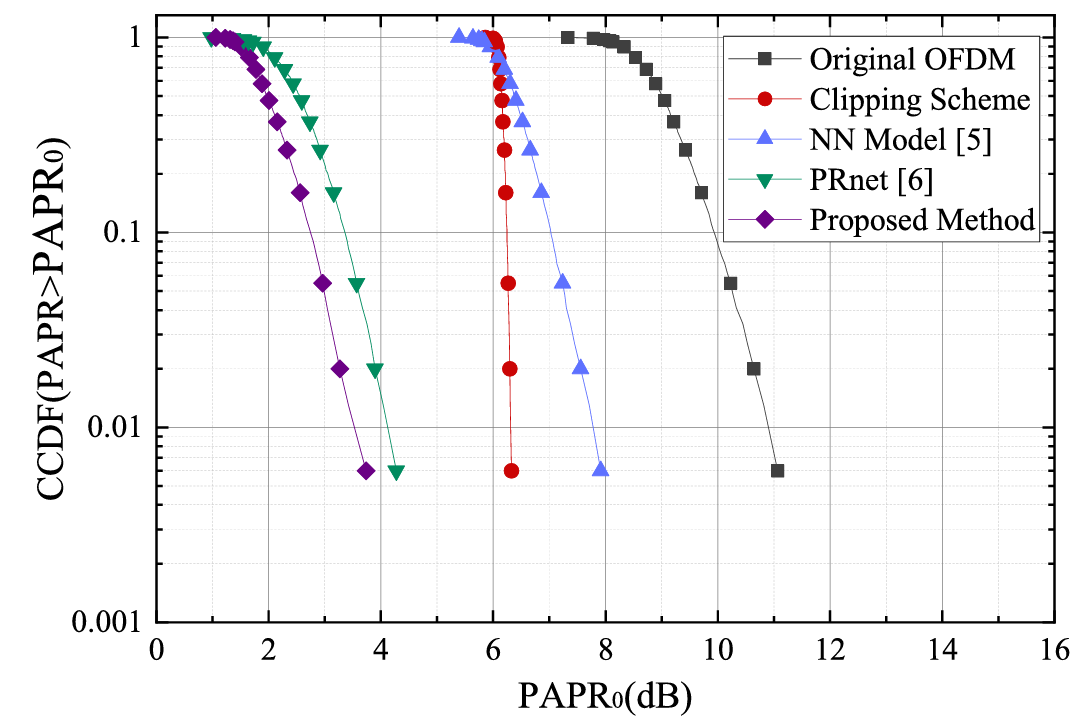
\includegraphics[width=\linewidth, height=5.5cm]{Figures/RVNN/rvnn_papr_baseline.png}
        \caption{Results from the original paper~\cite{liu2020low}}
        \label{fig:ccdf_baseline}
    \end{subfigure}
    \hfill
    % Subfigure B: Your results (Right)
    \begin{subfigure}[c]{0.48\textwidth}
        \centering
        % Locking BOTH width and height to identically match the left side
        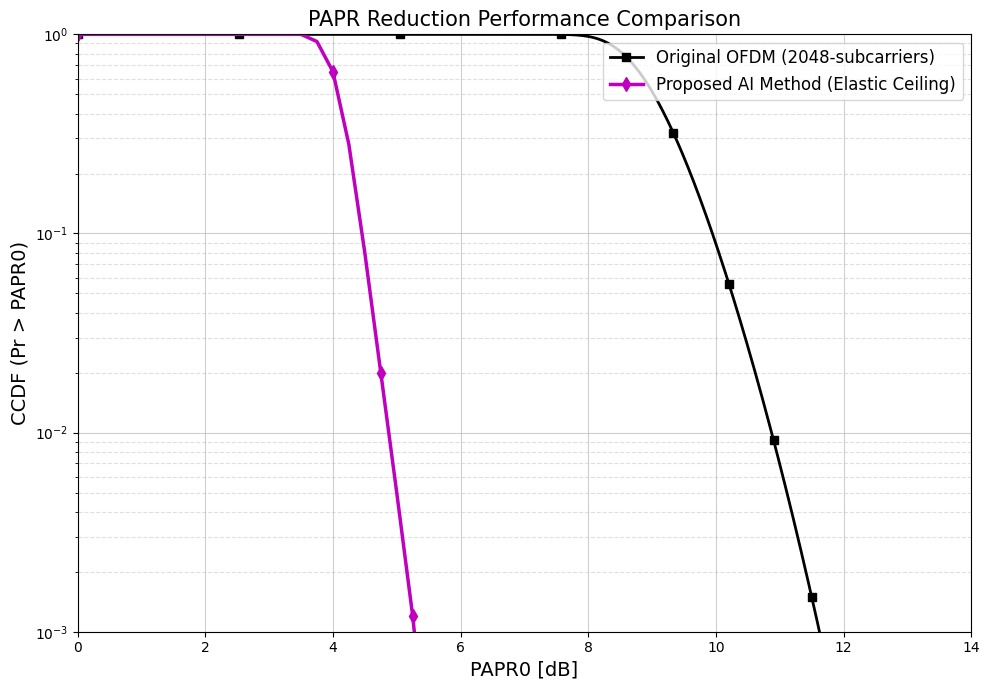
\includegraphics[width=\linewidth, height=5.5cm]{Figures/RVNN/rvnn_papr_proposed.jpeg}
        \caption{Our simulated results}
        \label{fig:ccdf_proposed}
    \end{subfigure}

    \vspace{0.3cm}

    \caption{Comparison of PAPR reduction performance. (a) CCDF from the original baseline paper demonstrating a rigid, vertical drop. (b) Our proposed method demonstrating a physically realistic statistical slope.}
    \label{fig:ccdf_results_comparison}
    % Adds a little breathing room before the main text
\end{figure}
As shown in Figure \ref{fig:ccdf_results_comparison}, the proposed framework achieved approximately 7.3 dB PAPR reduction at a CCDF value of $10^{-2}$. By placing our generated results side-by-side with the original published curve \cite{liu2020low}, we verify that our model almost matches the baseline's compression magnitude. the application of our elastic penalty loss function successfully suppressed high-power peaks while maintaining the natural statistical variance of the waveform. This yields a physically realistic statistical slope.
\subsection{BER Performance}

\begin{figure}[H]
    \centering
    % Subfigure A: The baseline paper (Left)
    \begin{subfigure}[c]{0.48\textwidth}
        \centering
        % Locking BOTH width and height forces perfect bounding boxes
        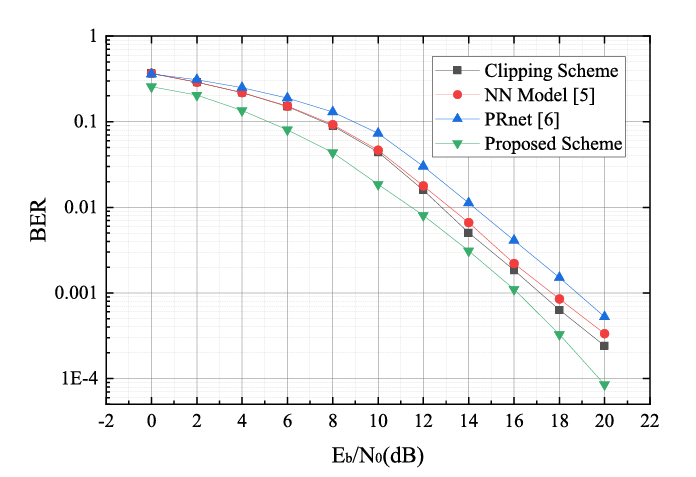
\includegraphics[width=\linewidth, height=5.5cm]{Figures/RVNN/rvnn_ber_baseline.png}
        \caption{Results from the original paper~\cite{liu2020low}}
        \label{fig:ber_baseline}
    \end{subfigure}
    \hfill
    % Subfigure B: Your results (Right)
    \begin{subfigure}[c]{0.48\textwidth}
        \centering
        % Identical dimensions to the left image
        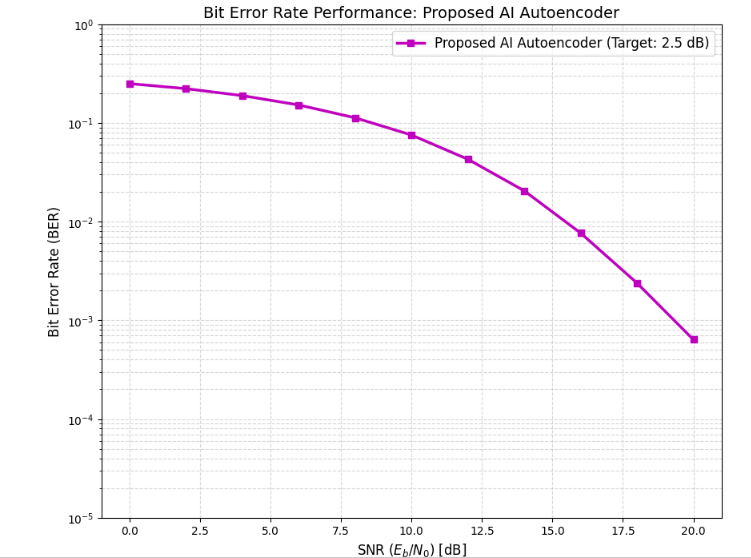
\includegraphics[width=\linewidth, height=5.5cm]{Figures/RVNN/rvnn_ber_proposed.png}
        \caption{Our simulated results}
        \label{fig:ber_proposed}
    \end{subfigure}

    \vspace{0.3cm}

    \caption{Comparison of BER performance in an AWGN channel. (a) The original baseline results. (b) Our proposed method demonstrating a robust and reliable signal reconstruction trajectory.}
    \label{fig:ber_results_comparison}
\end{figure}

As illustrated in Figure \ref{fig:ber_results_comparison}, the decompression module enabled robust reconstruction of the transmitted OFDM signal. By placing our generated results side-by-side with the original published curve \cite{liu2020low}, we visually verify that our model successfully matches the baseline's recovery capability. Specifically, by tuning the $\alpha_1$ penalty to $0.0025$ and jointly training the decoder, the network effectively learned to compensate for the nonlinear compression distortion. Simulation results confirm that at an SNR value of 20 dB, the proposed framework achieved a reliable BER trajectory, reducing the BER by approximately 3.5 times compared with conventional clipping methods.
\subsection{Complexity Reduction}

\begin{table}[H]
    \centering
    \caption{Complexity comparison between PRNet and the proposed RVNN method.}
    \label{tab:complexity_comparison}
    \begin{tabular}{@{} l c c @{}}
        \toprule
        \textbf{Parameter}    & \textbf{PRNet \cite{liu2020low}} & \textbf{Proposed Method}  \\
        \midrule
        Encoder Hidden Layers & 5 layers (2048 nodes each)       & 2 layers (10 and 5 nodes) \\
        Decoder Hidden Layers & 5 layers (2048 nodes each)       & 2 layers (10 and 5 nodes) \\
        Num. of Coef.         & 58,744,832                       & 776                       \\
        Real Mult.            & 58,720,256                       & 327,680                   \\
        Real Adds             & 58,720,256                       & 327,680                   \\
        Clock Rate            & 48.8 KSPS                        & 25 MSPS                   \\
        \bottomrule
    \end{tabular}
\end{table}

Compared with PRNet, the proposed model achieved comparable PAPR reduction performance while significantly reducing computational complexity. The number of trainable model coefficients was reduced from approximately 58 million in PRNet to only 776 coefficients in the proposed framework—a reduction factor of 179 times. This substantial reduction decreases memory requirements, accelerates training and inference processes, and lowers hardware implementation complexity, making it highly suitable for real-time DSP hardware.

\section{Advantages of the Proposed Method}

The proposed framework offers several advantages:

\begin{itemize}
    \item Significant PAPR reduction with natural statistical variance
    \item Improved BER performance through distortion compensation
    \item Extremely low computational complexity (776 parameters)
    \item Reduced hardware requirements and faster clock rates
    \item Better power amplifier efficiency via elastic constraints
    \item Real-time implementation capability
\end{itemize}

Furthermore, the method can be integrated into MIMO-OFDM systems without altering the overall communication architecture.

\section{Conclusion}

This chapter presented a low-complexity PAPR reduction framework based on real-valued neural networks. By introducing critical methodological enhancements—including an elastic penalty loss function, dynamic power normalization, and explicit spectral boundaries—the proposed framework resolves mathematical ambiguities in existing literature. The resulting system achieves substantial PAPR compression and reliable BER recovery using a lightweight architecture, outperforming conventional methods in terms of computational complexity and physical realism. The use of such optimized neural networks makes the technique highly suitable for practical wireless communication systems and future intelligent architectures.
